\documentclass[a4paper,oneside,14pt]{extarticle}

\usepackage{cmap} % Улучшенный поиск русских слов в полученном pdf-файле
\usepackage[T2A]{fontenc} % Поддержка русских букв
\usepackage[utf8]{inputenc} % Кодировка utf8
\usepackage[english,russian]{babel} % Языки: русский, английский

\usepackage[14pt]{extsizes}

\usepackage{graphicx}
\usepackage{multirow}

\usepackage{tikz}
\usetikzlibrary{shapes, shapes.geometric, arrows, arrows.meta, positioning}

\usepackage{caption}
\captionsetup{labelsep=endash}
\captionsetup[figure]{name={Рисунок}}

\usepackage{amsmath}
\usepackage{amsfonts}

\usepackage{geometry}
\geometry{left=30mm}
\geometry{right=10mm}
\geometry{top=20mm}
\geometry{bottom=20mm}

\usepackage{enumitem}

\usepackage{tabularx}
\usepackage{longtable}
\usepackage{adjustbox}
\usepackage{threeparttable}

% Переопределение стандартных \section, \subsection, \subsubsection по ГОСТу;
\usepackage{titlesec}[explicit]
\titleformat{name=\section,numberless}[block]{\normalfont\large\bfseries\centering}{}{0pt}{}
\titleformat{\section}[block]{\normalfont\large\bfseries}{\thesection}{1em}{}
\titlespacing\section{\parindent}{*4}{*4}

\titleformat{\subsection}[hang]
{\bfseries\large}{\thesubsection}{1em}{}
\titlespacing\subsection{\parindent}{*2}{*2}

\titleformat{\subsubsection}[hang]
{\bfseries\large}{\thesubsubsection}{1em}{}
\titlespacing\subsubsection{\parindent}{*2}{*2}

\usepackage{url}

% Переопределение их отступов до и после для 1.5 интервала во всем документе
\usepackage{setspace}
\onehalfspacing % Полуторный интервал
\frenchspacing
\setlength\parindent{1.25cm}

\usepackage{indentfirst} % Красная строка

% Настройки оглавления
\usepackage{xcolor}
\usepackage{multirow}

% Гиперссылки
\usepackage[pdftex]{hyperref}
\hypersetup{hidelinks}

% Дополнительное окружения для подписей
\usepackage{array}
\newenvironment{signstabular}[1][1]{
	\renewcommand*{\arraystretch}{#1}
	\tabular
}{
	\endtabular
}

\usepackage{enumitem} 
\setenumerate[0]{label=\arabic*)} % Изменение вида нумерации списков
\renewcommand{\labelitemi}{---}

% Листинги 
\usepackage{courier}
\usepackage{listings}
\usepackage{chngcntr} % Listings counter within section set main.tex after begin document
\usepackage{float} % Place figures anywhere you want; ignore floating
\floatstyle{plaintop}
\newfloat{code}{H}{myc}

% Для листинга кода:
\lstset{
	basicstyle=\small\ttfamily,			% размер и начертание шрифта для подсветки кода
	language=C++,   					% выбор языка для подсветки	
	numbers=left,						% где поставить нумерацию строк (слева\справа)
	numbersep=5pt,
	% stepnumber=1,						% размер шага между двумя номерами строк
	xleftmargin=17pt,
	% showstringspaces=false,
	numbersep=5pt,						% как далеко отстоят номера строк от подсвечиваемого кода
	frame=single,						% рисовать рамку вокруг кода
	tabsize=4,							% размер табуляции по умолчанию равен 4 пробелам
	captionpos=b,						% позиция заголовка вверху [t] или внизу [b]
	breaklines=true,					
	breakatwhitespace=true,				% переносить строки только если есть пробел
	escapeinside={\#*}{*)},				% если нужно добавить комментарии в коде
	inputencoding=utf8x,
	backgroundcolor=\color{white},
	numberstyle=,%\tiny,					    % размер шрифта для номеров строк
	keywordstyle=\color{blue},
	stringstyle=\color{red!90!black}, % color of text in ""
	commentstyle=\color{green!50!black}
}
\lstset{
 morekeywords={size_t, likely}
}

\lstset{
	literate=
	{а}{{\selectfont\char224}}1
	{б}{{\selectfont\char225}}1
	{в}{{\selectfont\char226}}1
	{г}{{\selectfont\char227}}1
	{д}{{\selectfont\char228}}1
	{е}{{\selectfont\char229}}1
	{ё}{{\"e}}1
	{ж}{{\selectfont\char230}}1
	{з}{{\selectfont\char231}}1
	{и}{{\selectfont\char232}}1
	{й}{{\selectfont\char233}}1
	{к}{{\selectfont\char234}}1
	{л}{{\selectfont\char235}}1
	{м}{{\selectfont\char236}}1
	{н}{{\selectfont\char237}}1
	{о}{{\selectfont\char238}}1
	{п}{{\selectfont\char239}}1
	{р}{{\selectfont\char240}}1
	{с}{{\selectfont\char241}}1
	{т}{{\selectfont\char242}}1
	{у}{{\selectfont\char243}}1
	{ф}{{\selectfont\char244}}1
	{х}{{\selectfont\char245}}1
	{ц}{{\selectfont\char246}}1
	{ч}{{\selectfont\char247}}1
	{ш}{{\selectfont\char248}}1
	{щ}{{\selectfont\char249}}1
	{ъ}{{\selectfont\char250}}1
	{ы}{{\selectfont\char251}}1
	{ь}{{\selectfont\char252}}1
	{э}{{\selectfont\char253}}1
	{ю}{{\selectfont\char254}}1
	{я}{{\selectfont\char255}}1
	{А}{{\selectfont\char192}}1
	{Б}{{\selectfont\char193}}1
	{В}{{\selectfont\char194}}1
	{Г}{{\selectfont\char195}}1
	{Д}{{\selectfont\char196}}1
	{Е}{{\selectfont\char197}}1
	{Ё}{{\"E}}1
	{Ж}{{\selectfont\char198}}1
	{З}{{\selectfont\char199}}1
	{И}{{\selectfont\char200}}1
	{Й}{{\selectfont\char201}}1
	{К}{{\selectfont\char202}}1
	{Л}{{\selectfont\char203}}1
	{М}{{\selectfont\char204}}1
	{Н}{{\selectfont\char205}}1
	{О}{{\selectfont\char206}}1
	{П}{{\selectfont\char207}}1
	{Р}{{\selectfont\char208}}1
	{С}{{\selectfont\char209}}1
	{Т}{{\selectfont\char210}}1
	{У}{{\selectfont\char211}}1
	{Ф}{{\selectfont\char212}}1
	{Х}{{\selectfont\char213}}1
	{Ц}{{\selectfont\char214}}1
	{Ч}{{\selectfont\char215}}1
	{Ш}{{\selectfont\char216}}1
	{Щ}{{\selectfont\char217}}1
	{Ъ}{{\selectfont\char218}}1
	{Ы}{{\selectfont\char219}}1
	{Ь}{{\selectfont\char220}}1
	{Э}{{\selectfont\char221}}1
	{Ю}{{\selectfont\char222}}1
	{Я}{{\selectfont\char223}}1
}

% Работа с изображениями и таблицами; переопределение названий по ГОСТу
\usepackage{caption}
\captionsetup[figure]{name={Рисунок},labelsep=endash}
\captionsetup[table]{singlelinecheck=false, labelsep=endash}

\usepackage[justification=centering]{caption} % Настройка подписей float объектов	

\usepackage{csvsimple}

\usepackage{ulem} % Нормальное нижнее подчеркивание
\usepackage{hhline} % Двойная горизонтальная линия в таблицах
\usepackage[figure,table]{totalcount} % Подсчет изображений, таблиц
\usepackage{rotating} % Поворот изображения вместе с названием
\usepackage{lastpage} % Для подсчета числа страниц

\makeatletter
\renewcommand\@biblabel[1]{#1.} % [1] -> 1. in bibliography
\makeatother

\usepackage{ragged2e} % Перенос слов на следующую строку
\usepackage{pdfpages}

\usepackage{blindtext}

\renewcommand{\underset}[2]{\ensuremath{\mathop{\mbox{#2}}\limits_{\mbox{\scriptsize #1}}}} % Use \underset in normal environment, not only in math
\NewDocumentCommand{\ulinetext}{O{3cm} O{c} m m} % O - optional; m - mandatory
{\underset{#3}{\uline{\makebox[#1][#2]{#4}}}}

% \usepackage[
%     backend=biber,
% 	style=gost-numeric,
% 	% style=numeric-comp,
% 	language=auto,
% 	autolang=other,
% 	sorting=none
% ]{biblatex}
% \addbibresource{bibliography.bib}
% \usepackage{xparse} % \NewDocumentCommand for creating custom commands
% \NewDocumentCommand{\printbib}{m}
% {\printbibliography[title={#1}]\addcontentsline{toc}{section}{#1}}


\begin{document}

\def\coursename{Моделирование}
\def\labnumber{\textbf{{1}}}
\def\myname{Рунов К.А.}
\def\teachername{Рудаков И.В.}
\def\mygroup{ИУ7-74Б}

\begin{titlepage}
    \newgeometry{left=2cm, right=1cm, top=2.5cm, bottom=2.5cm}
    \fontsize{12pt}{12pt}\selectfont

    \noindent
    \begin{center}
        % \fbox
        % \begin{tabular}{|l|r|}
        % {
            % \hline
            \begin{minipage}{0.12\textwidth}
                
\includegraphics[width=\linewidth]{img/bmstu_logo.jpg}
            \end{minipage}
            \hfill
            % &
            % \hspace{0.2cm}
            \begin{minipage}{0.85\textwidth}\centering\bfseries
                {
                    \linespread{1}\selectfont
                    \vspace{0.1cm}
                    % \textsc
                    {Министерство науки и высшего образования~Российской~Федерации}

                    % \textsc
                    {Федеральное~государственное~бюджетное~образовательное~учреждение высшего образования}

                    % \textsc
                    {<<Московский государственный технический университет имени~Н.~Э.~Баумана (национальный~исследовательский~университет)>>}

                    % \textsc
                    {(МГТУ им. Н.~Э.~Баумана)}
                    \vspace{0.1cm}
                }
            \end{minipage}
            % \\
            % \hline
        % }
        % \end{tabular}

        \vspace{0.2cm}
        \rule{\linewidth}{2.8pt}
        \rule[3ex]{\linewidth}{1pt}

        \begin{flushleft}
            {ФАКУЛЬТЕТ \uline{<<Информатика и системы управления>> \hfill}}

            \vspace{0.5cm}

            {КАФЕДРА \uline{<<Программное обеспечение ЭВМ и информационные технологии>> \hfill}}
        \end{flushleft}

        % \vspace{1cm}
        \vfill

        {
            \Large{\textbf{
                % \bolduline
                {ОТЧЕТ ПО ЛАБОРАТОРНОЙ РАБОТЕ №\labnumber}
            }}

            \Large{\textbf{
                % \bolduline
                {по курсу <<\coursename>>}
            }}

            %\Large{\textbf{
            %    % \bolduline
            %    {на тему:}
            %}}

            %\large{<<\labtheme>>}

            \vspace{0.5cm}
        }

        \vspace{0.5cm}

        \fontsize{14pt}{14pt}\selectfont

        \vfill

        \begin{flushleft}
            % {Студент \uline{Рунов Константин Алексеевич \hfill}}
            {Студент \uline{\myname \hfill}}

            \vspace{0.5cm}

            {Группа\,\, \uline{\mygroup \hfill}}

            \vspace{0.5cm}

            % {Оценка (баллы) \uline{\hfill}}

            % \vspace{0.5cm}

            \vfill

            % {Преподаватель \hfill \ulinetext[4cm]{(Подпись, дата)}{} \ulinetext[4cm]{}{Волкова Л.~Л.}}
            % {Преподаватели \uline{Волкова Лилия Леонидовна, Строганов Дмитрий Владимирович \hfill}}
            %{Преподаватели \uline{\teachers \hfill}}

            % \vspace{0.5cm}

            {Студент \hfill \ulinetext[4cm]{(Подпись, дата)}{} \ulinetext[4cm]{(Фамилия И.О.)}{\myname}}

            \vspace{0.5cm}

            {Преподаватель \hfill \ulinetext[4cm]{(Подпись, дата)}{} \ulinetext[4cm]{(Фамилия И.О.)}{\teachername}}

            \vspace{0.5cm}

        \end{flushleft}

        \vfill

        \the\year\ г.

    \end{center}
\end{titlepage}


\setcounter{page}{2}
%\renewcommand{\contentsname}{СОДЕРЖАНИЕ}
%\tableofcontents

\section{Теоретическая часть}

\subsection{Равномерное распределение}

Случайная величина имеет равномерное распределение на отрезке $[a, b]$, если ее функция плотности распределения вероятностей
\[
f(x) =
\begin{cases}
    \begin{array}{c l}
        \dfrac{1}{b - a}, & a \leq x \leq b; \\
        0, & x < a \text{ или } x > b.
    \end{array}
\end{cases}
\]

Ее функция распределения в этом случае определяется выражением
\[
F(x) =
\begin{cases}
    \begin{array}{c l}
    0, & x < a; \\
    \dfrac{x - a}{b - a}, & a \leq x \leq b; \\
    1, & x > b.
    \end{array}
\end{cases}
\]

\subsection{Нормальное распределение}

Случайная величина имеет нормальное распределение, если ее функция плотности распределения вероятностей 
\[
    f(x) = \dfrac{1}{\sigma\sqrt{2\pi}}e^{\displaystyle -\frac{(x-m)^2}{2\sigma^2}} \hspace{0.5cm} (m \in \mathbb{R},\ \sigma > 0).
\]

Функция нормального распределения имеет вид
\[
    F(x) = \dfrac{1}{\sigma\sqrt{2\pi}} \int\displaylimits_{-\infty}^{x} e^{\displaystyle -\frac{(x - m)^2}{2\sigma^2}} dx.
\]

\subsection{Распределение Пуассона}

Дискретная случайная величина $X$ распределена по закону Пуассона, если она принимает целые неотрицательные значения с вероятностями
\[
    \mathrm{P}\{X = i\} = P(i;\, \lambda) = \dfrac{\lambda^i}{i!} e^{\displaystyle -\lambda}, \hspace{1cm} i = 0, 1, \dots
\]

Ее функция распределения
\[
    F(k;\, \lambda) = \mathrm{P}\{X \leq k\} = \sum\displaylimits_{i = 0}^k P(i;\, \lambda) = e^{\displaystyle -\lambda} \sum\displaylimits_{i = 0}^k \dfrac{\lambda^i}{i!}.
\]

\subsection{Распределение Эрланга}

Распределение Эрланга --- частный случай Гамма распределения, когда параметр $k$ является целым числом.

Случайная величина имеет Эрланговское распределение, если ее функция плотности распределения вероятностей 
\[
    f(x) =
    \begin{cases}
        \begin{array}{c l}
            x^{k-1}\dfrac{e^{-x/\theta}}{\theta^k \,(k-1)!}, & x \geq 0; \\
            0, & x < 0.
        \end{array}
    \end{cases}
\]

Функция распределения Эрланга
\[
    F(x; k, \theta) =
    \begin{cases}
        \begin{array}{c l}
            1 - e^{-x/\theta} \displaystyle \sum\displaylimits_{i = 0}^{k - 1} \dfrac{x^i}{\theta^i \,i!}, & x \geq 0; \\
            0, & x < 0.
        \end{array}
    \end{cases}
\]

\newpage

\section{Практическая часть}

\subsection{Равномерное распределение}

\begin{figure}[H]
	\centering
	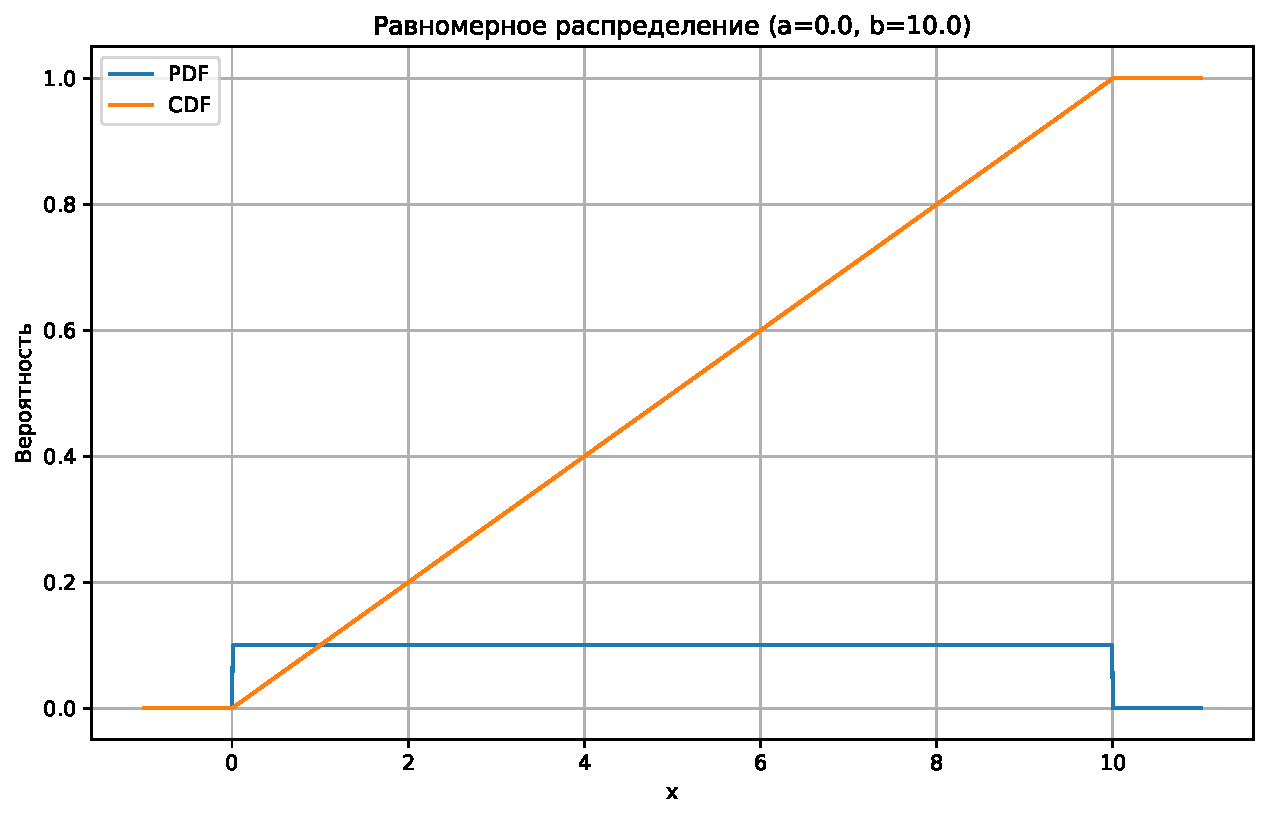
\includegraphics[scale=0.6]{img/th_regular.pdf}
	\caption{Равномерное распределение --- функция распределения и функция плотности распределения вероятностей}
	\label{fig:}
\end{figure}

\begin{figure}[H]
	\centering
	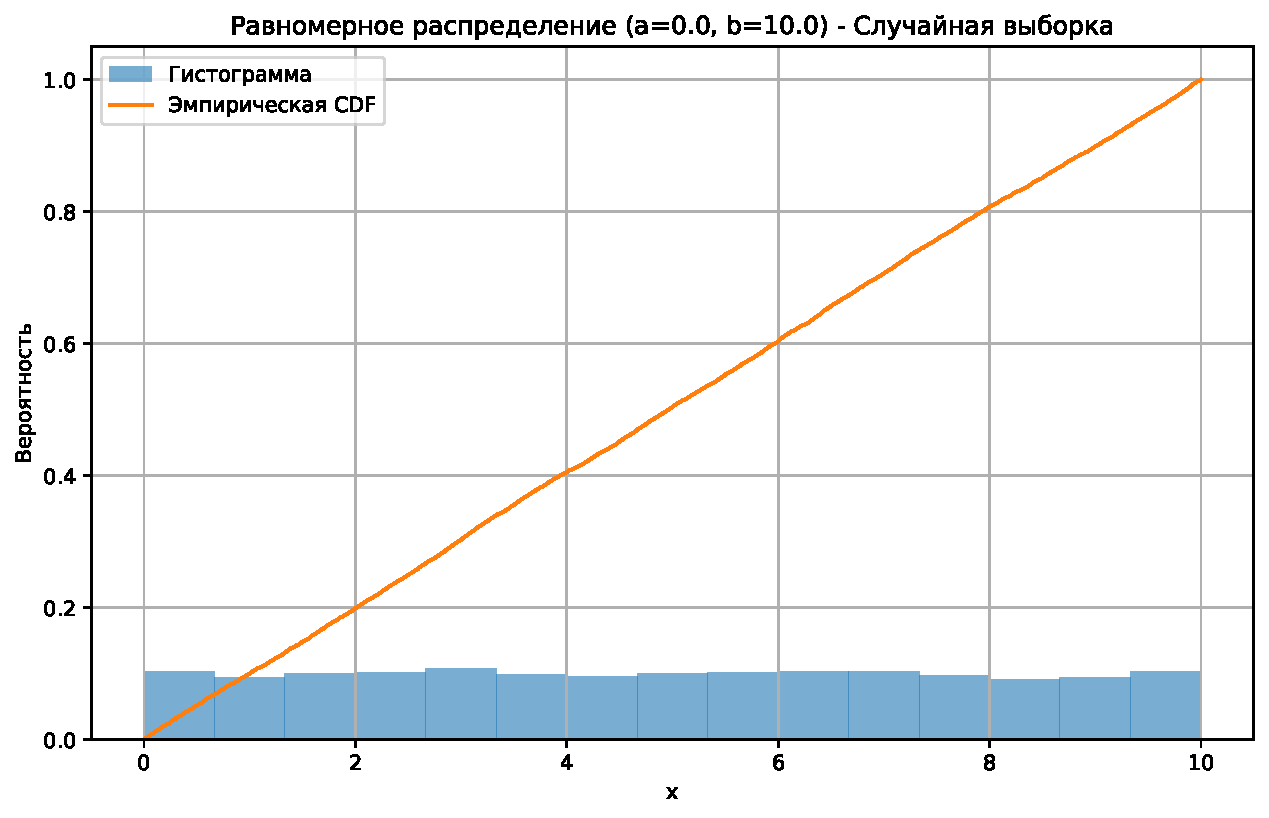
\includegraphics[scale=0.6]{img/emp_regular.pdf}
	\caption{Равномерное распределение --- эмпирическая функция распределения и гистограмма}
	\label{fig:}
\end{figure}

\subsection{Нормальное распределение}

\begin{figure}[H]
	\centering
	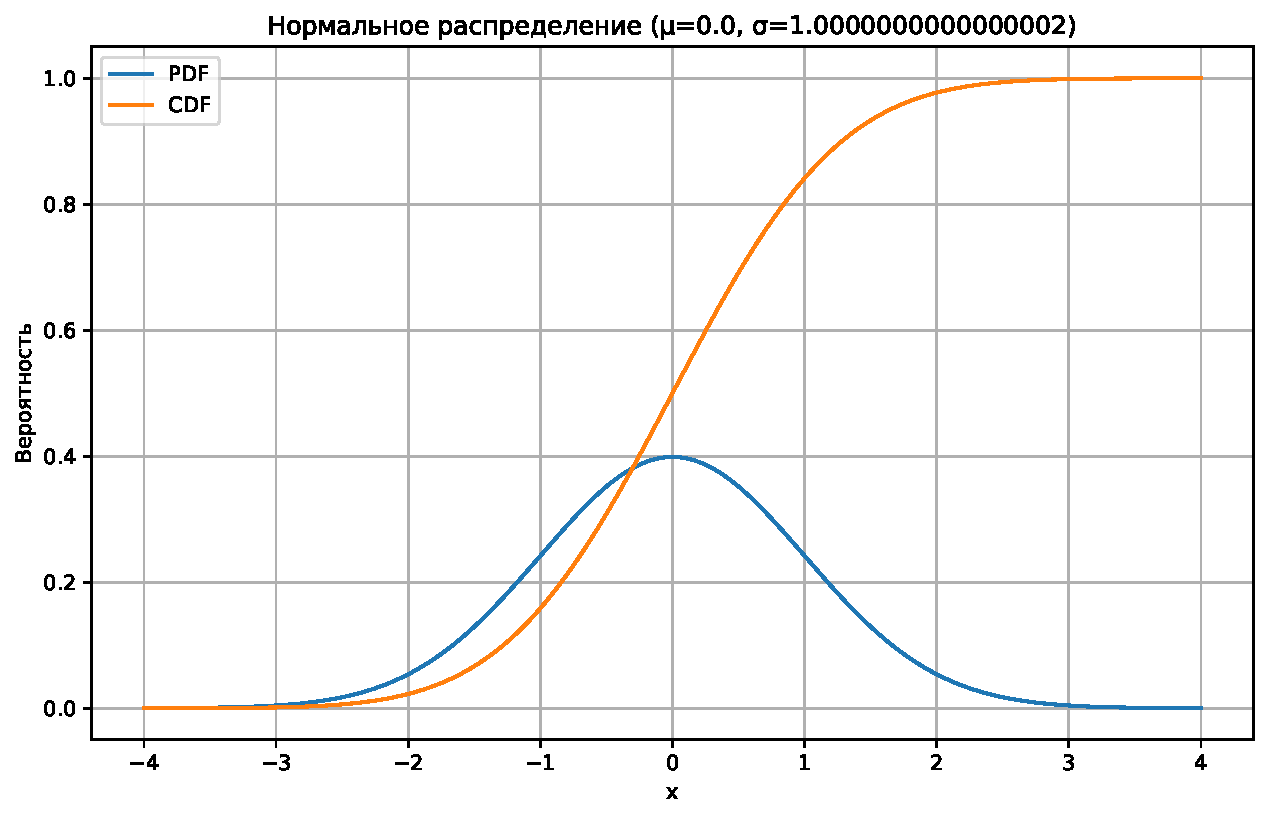
\includegraphics[scale=0.7]{img/th_normal.pdf}
	\caption{Нормальное распределение --- функция распределения и функция плотности распределения вероятностей}
	\label{fig:}
\end{figure}

\begin{figure}[H]
	\centering
	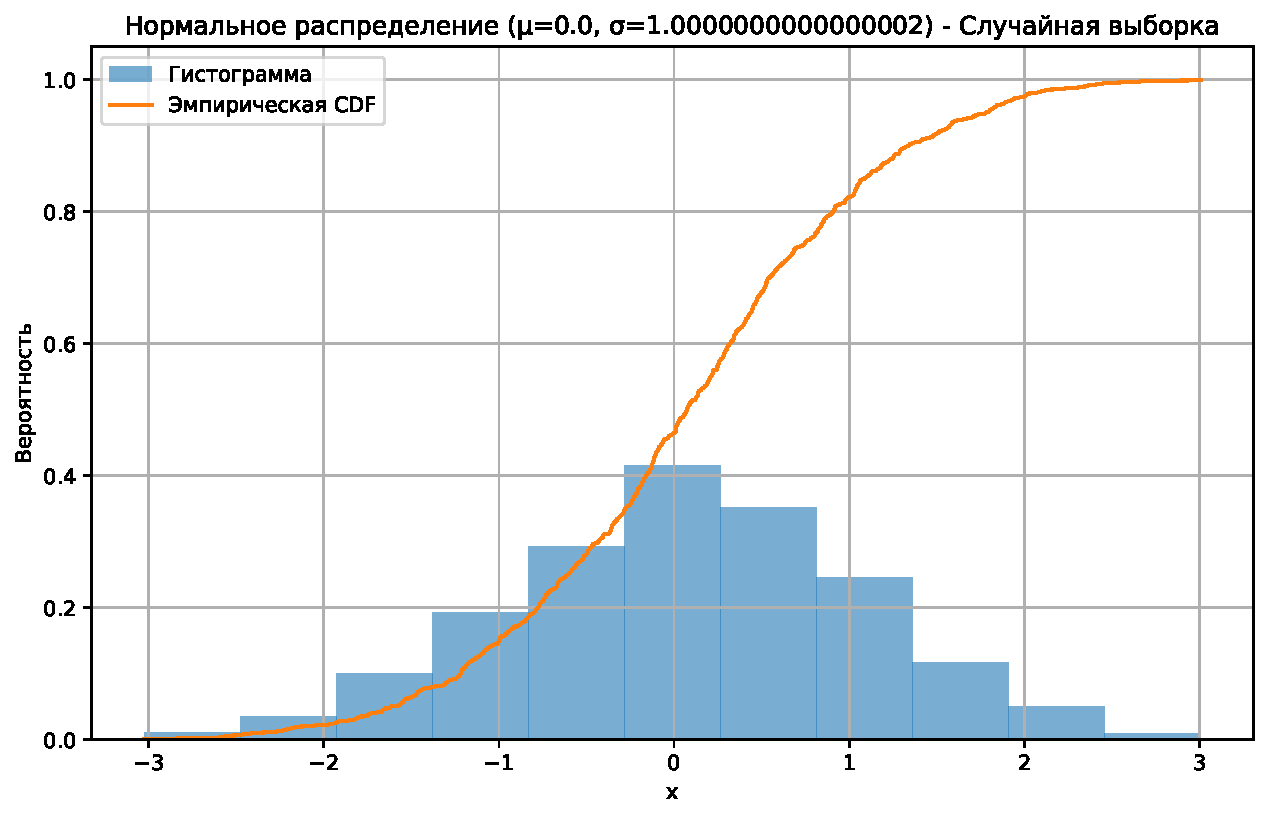
\includegraphics[scale=0.7]{img/emp_normal.pdf}
	\caption{Нормальное распределение --- эмпирическая функция распределения и гистограмма}
	\label{fig:}
\end{figure}

\subsection{Распределение Пуассона}

\begin{figure}[H]
	\centering
	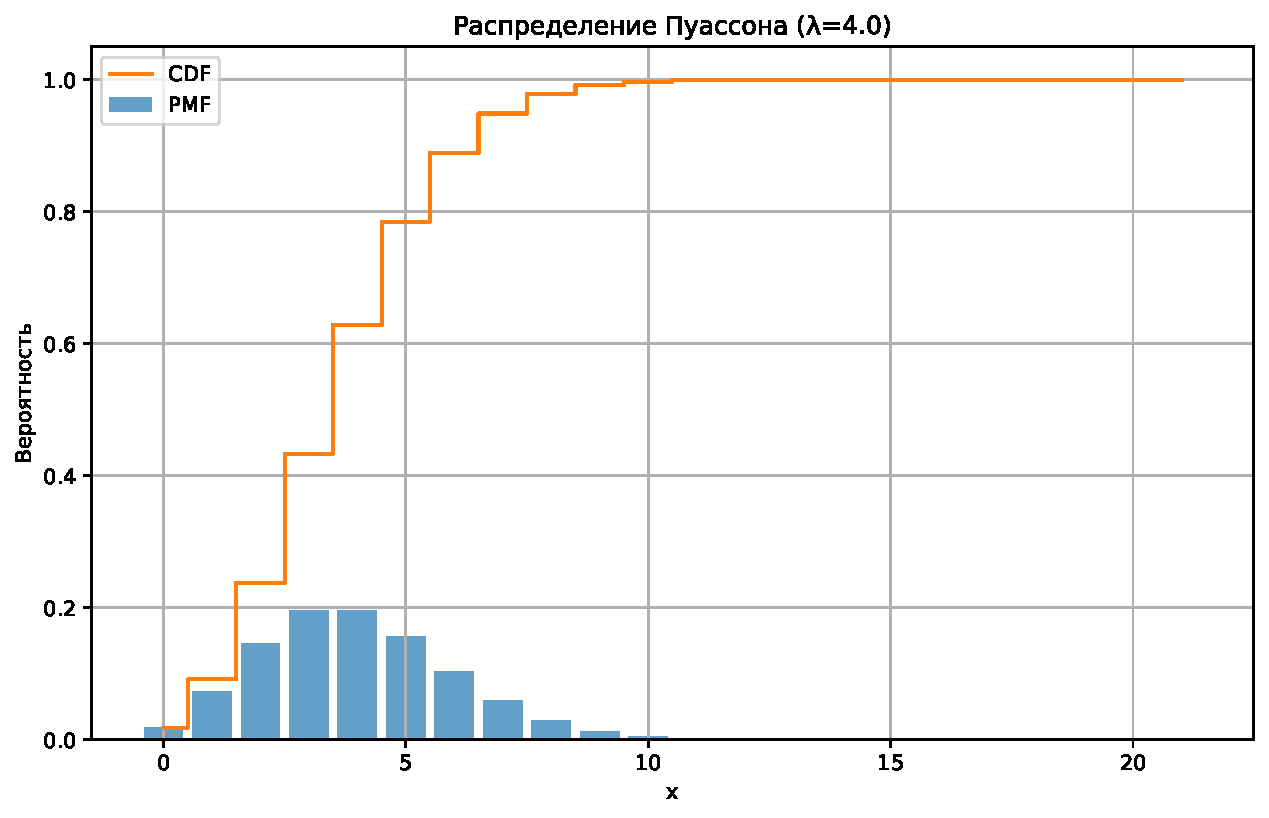
\includegraphics[scale=0.7]{img/th_poisson.pdf}
	\caption{Пуассоновское распределение --- функция распределения и функция плотности распределения вероятностей}
	\label{fig:}
\end{figure}

\begin{figure}[H]
	\centering
	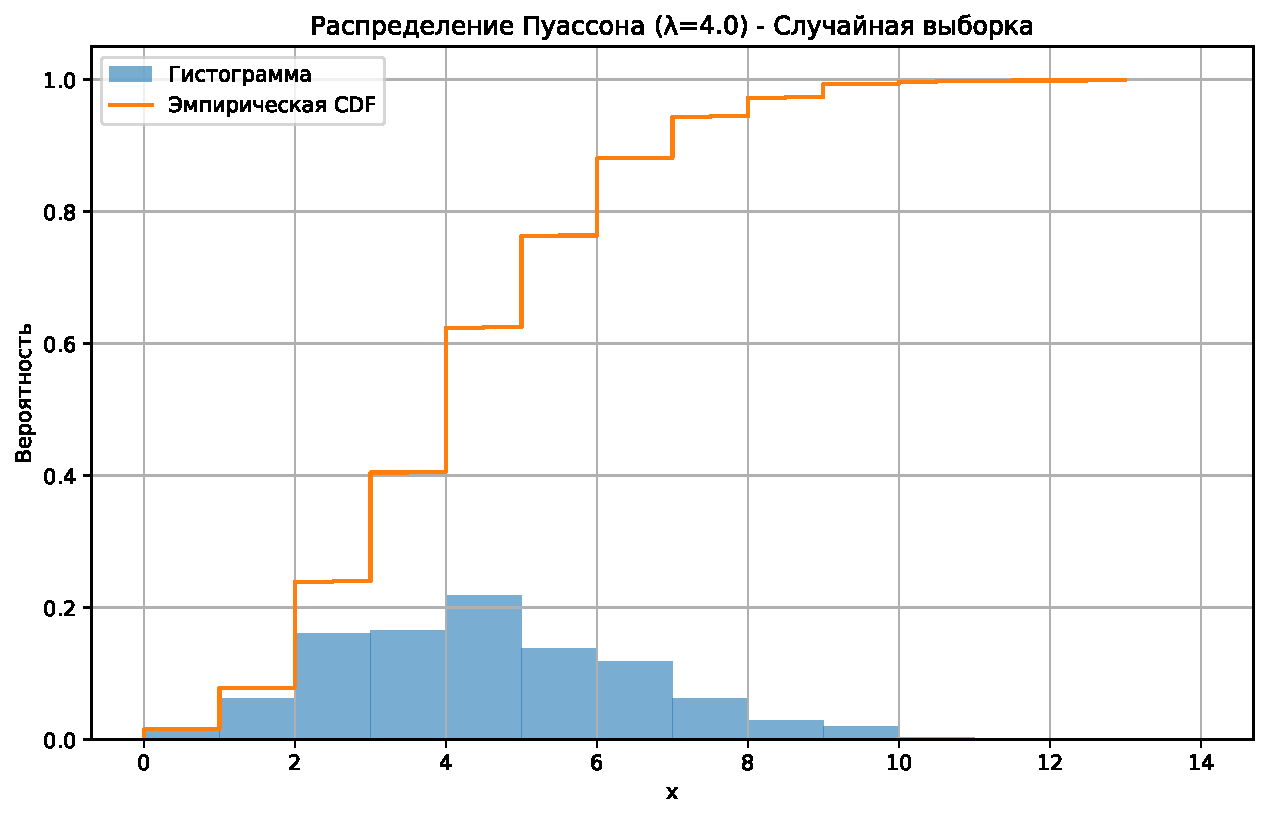
\includegraphics[scale=0.7]{img/emp_poisson.pdf}
	\caption{Пуассоновское распределение --- эмпирическая функция распределения и гистограмма}
	\label{fig:}
\end{figure}

\subsection{Распределение Эрланга}

\begin{figure}[H]
	\centering
	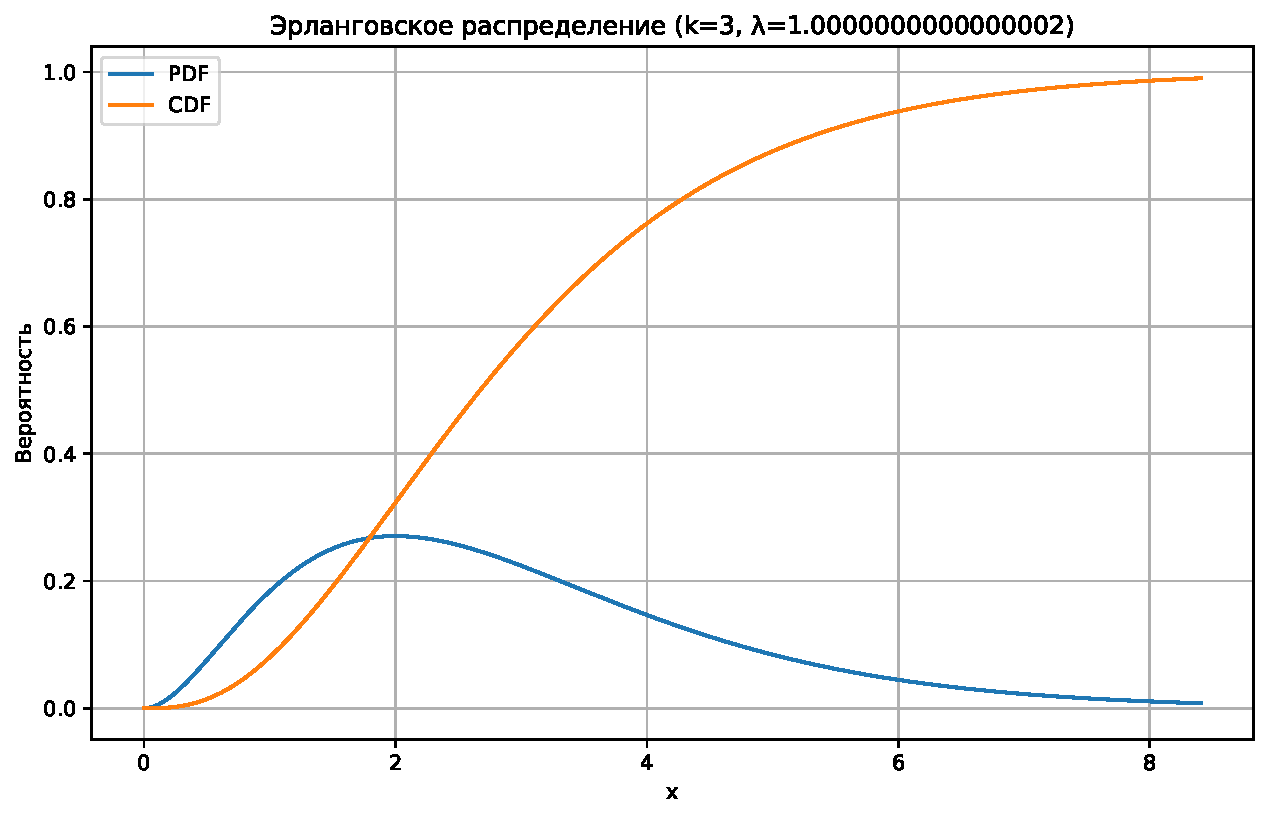
\includegraphics[scale=0.7]{img/th_erlang.pdf}
	\caption{Эрланговское распределение --- функция распределения и функция плотности распределения вероятностей}
	\label{fig:}
\end{figure}

\begin{figure}[H]
	\centering
	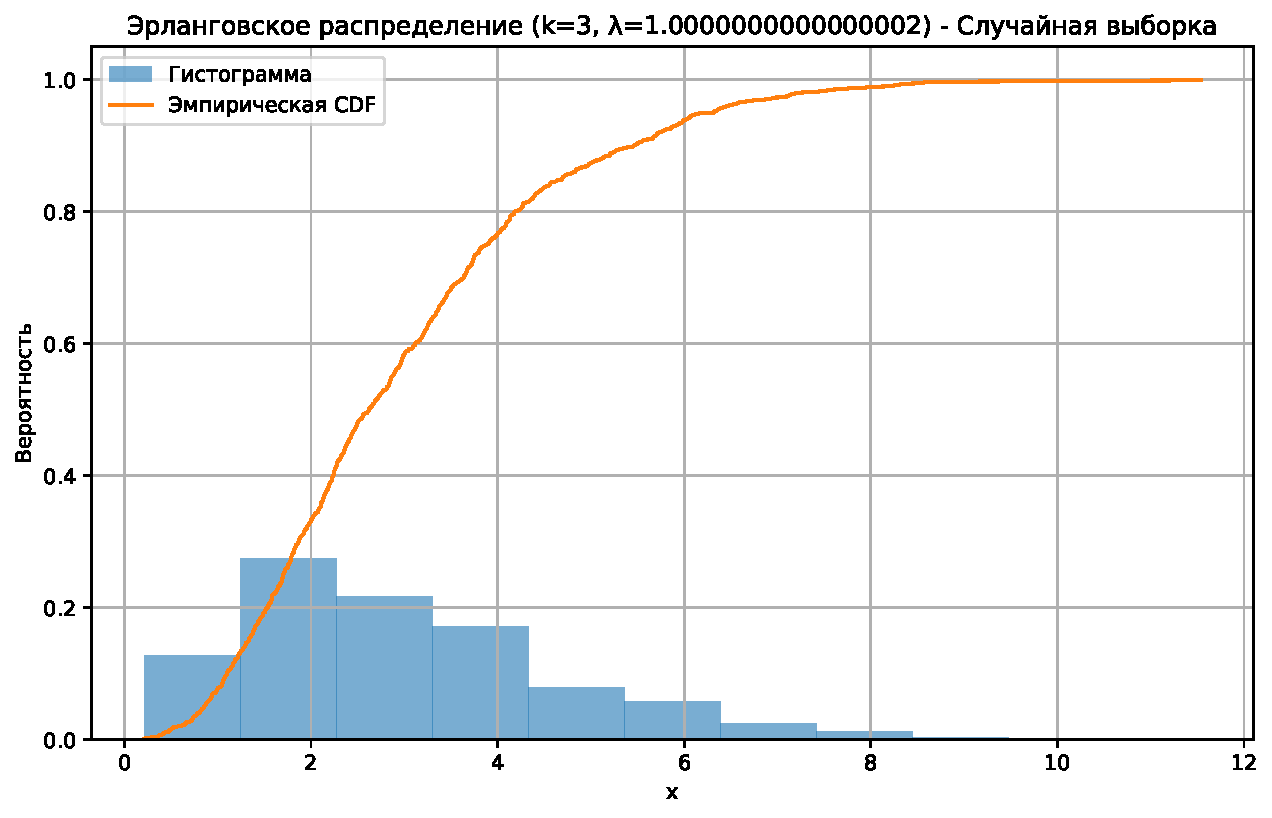
\includegraphics[scale=0.7]{img/emp_erlang.pdf}
	\caption{Эрланговское распределение --- эмпирическая функция распределения и гистограмма}
	\label{fig:}
\end{figure}

\end{document}
